%!TEX root = disclosure_game.tex
\section{Disclosure Game Model Development}
\label{app:model_description}

This appendix provides a more in depth exploration of the model development process, beginning by deriving a game to serve as the basis for the model, and decision problems.

A game, in the game theoretic sense, this can be any interaction where the result for one person is dependent on the actions of another. In this scenario, the result for the woman would seem dependent on whether the midwife chooses to refer them for specialist support (although naturally the reality can only be thought of in terms of risk mitigation), and conversely, the right choice for the midwife is somewhat contingent on what the woman is willing to tell them.

A very simple way to represent this would be a game with two players, who both have two possible moves - ask for help, or not; and refer, or not (fig \ref{fig:simplest_game}). Since both parties are invested in the outcome of the pregnancy, we might allow them to share the same payoff if everything ends well.


\begin{figure}[H]
\sidecaption
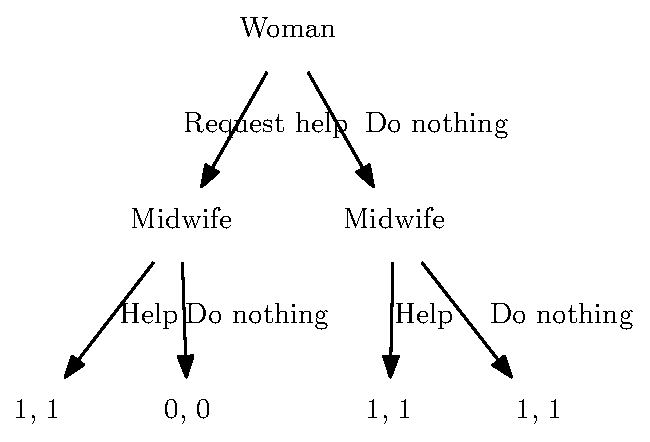
\includegraphics[width=7cm]{figures/simplest_game}
\caption{A very simple two player game. The only time things in this very restricted world obviously end poorly, is if the woman asks for help but does not get any. This implies that a rational player would always refer if asked for help, and is indifferent otherwise - in other words, there are three possible Nash equilibriums.}
\label{fig:simplest_game}
\end{figure}

The first complication, is that there should be differentiation between referring, and doing nothing because specialist treatment incurs a cost. We can modify the payoffs to reflect this, by reducing the midwife's payoffs when they refer. If the cost of referring is less than the value of a good outcome, then the effect of this is to make the only rational choice when not asked for help is to do nothing.

This simple game is however not very informative, and clearly neglects much of the nuance of the scenario. The wider difficulty here is that the real outcome depends on an attribute of one of the players, rather than their moves. In this case, we would expect the right choices to depend on the alcohol consumption of the woman, rather than entirely on what they have claimed about it.
To reflect this, we would need different variations on the same game to reflect this attribute. 

To resolve this, we can do exactly that, and cast it as a signalling game. We make the simplifying assumption that a woman may have one of only three drinking patterns - light\footnote{Or abstinent, the extent of alcohol consumption being such that it would generally be felt to pose essentially no risk.}, moderate, or heavy. Each of these types of player, will play a different game. This also introduces a third player, who we will call nature. Nature takes the first move, and decides the type of the woman according to some probability distribution; in this case we will allow the probability of types to be uniform. 
This changes the dynamics of play substantially, since the midwife can no longer be certain of which game they are playing, and hence which move yields the best outcome. We must also amend the moves, and payoffs slightly. The woman now claims to be one of the types, and may send a signal to say, for example, that they are a heavy drinker. We will also modify the common payoffs to allow light drinkers to get the best outcome no matter what, and moderate and heavy types to get the best outcome only if referred. We can also differentiate between the consequences of not getting help for these types by letting heavy drinkers have a very negative outcome, and moderate drinkers a slight one (fig \ref{fig:less_simple}).

\begin{figure}[H]
\begin{adjustbox}{center}
\includegraphics[width=78mm]{figures/less_simple_game}
\end{adjustbox}
\sidecaption{A less simple two player game.}

\label{fig:less_simple}
\end{figure}

At this point, the game becomes challenging to analyse from a Nash equilibrium perspective (there are several hundred). But, having raised to issue of stigma, we would also like incorporate this in the game. A possible approach to this is similar to the drinking behaviour of the women, and lets midwives have a type as well, corresponding to how judgemental they are when receiving signals: non-judgemental, moderately judgemental, and harshly judgemental. The expression of this judgement is not a matter of choice on their part, and is assumed to have no impact on their clinical response. Nature now has an additional move, to choose the type of the midwife, and we add costs for sending moderate and heavy signals. A heavy signal to a harshly judgemental midwife adds a heavy cost, and a moderate cost from a moderate midwife. The resulting game might reasonably be said to be intractable.

At this juncture, we do not gain much further from the game representation, and instead separate it into multiple decision problems. 

Breaking the game down into separate decision problems can be achieved by treating the moves of the other players as a chance node, and omitting moves by nature that are known to them. For women, there are two such nodes, corresponding to the move by nature determining the type of midwife they play against, and the midwife's action. Midwives have simpler problem with only a single chance node, because the woman's move is known to them. Figure \ref{fig:decision_problems} shows the structure of the resulting decision problems. Note that there are in fact three distinct decision problems for the three types of woman, since the move by nature determining their type is known to them. 

\begin{figure}[H]
\centering
\subfloat[Women (heavy drinkers)]{\includegraphics[width=119mm]{figures/women_influence}}
\vskip\baselineskip
\subfloat[Midwives]{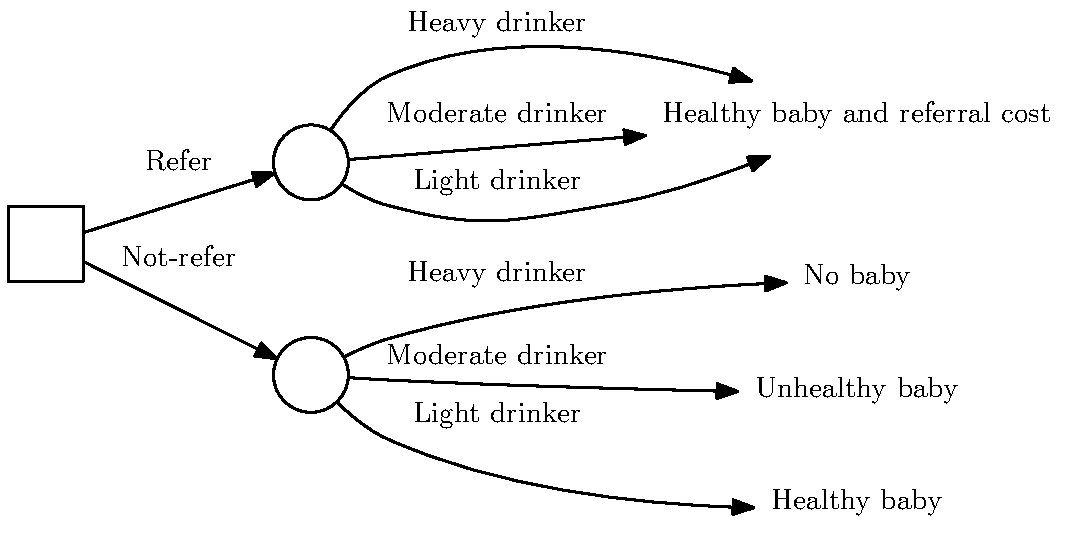
\includegraphics[width=119mm]{figures/mw_influence}}
\caption{Influence diagrams, showing the game broken into two decision problems. Squares indicate a decision node, while circles are (from the perspective of the agent) chance nodes}

\label{fig:decision_problems}
\end{figure}


The precise structure of the decision problem is to some extent dependent on the decision rule in use, for example the Lexicographic heuristic rule is concerned only with a direct relationship between action and consequence. However, the literal translation from game to decision problem for women yields two chance nodes. As a result, solving this using the heuristic approach requires that the nodes be combined. By the same token, an arbitrarily complex problem could be resolved by rules without this limitation. This is significant, in that the decision problem is an individual agent's model of the situation, which might not be expected to correspond perfectly with the true situation.

From this position, simulating play, and augmenting the basic conjecture is easily achievable, since together the game, and the decision rules specify the basis for a simulation model. In the disclosure game case, we make additional stipulations on how many games agents play, order of play, the circumstances under which agents observe true types, and the structure of agent populations amongst others. 

\begin{comment}
At the end of a game, each player receives a payoff dependent on the actions and types of both players. Because both women and midwives have an interest in the outcome of the pregnancy, and would prefer a healthy baby, the payoff has a common interest component. Hence, both players receive a payoff based on the outcome of pregnancy, but women bear a social cost dependent on the signal they sent and the midwife's reaction to it. Similarly, midwives pay a cost if they refer to a specialist, mirroring the organisational cost of non-routine care. Table \ref{tab:Payoff-matrix} shows the three payoff matrices which together describe the game.



Taken together, this leads to a game tree that is relatively complex (figure \ref{fig:simple_tree} shows a simplified representation, with a detailed view of one branch in figure \ref{fig:zoom_tree}) even at the subgame level. 

As an example, consider the challenge faced by an agent of the heavy drinking type. In order to get the best health outcome, they must be referred and would ideally achieve this without paying any social cost at all. The best move depends on the type, and beliefs of the midwife. For example, a particularly unlucky scenario might be for the midwife to not only be of a harshly judgemental disposition, but to believe that no women really need to be referred. Even a relatively weak belief in this possibility can make the honest signal look like an unwarranted risk.

Rather than attempt to solve for equilibria, agents treat this two player game as taking place against nature, along the lines of adversarial risk analysis \citep{RiosInsua2009}. This effectively translates the game to a pair of decision problems (figure \ref{fig:decision_problems}), which agents attempt to resolve at each turn using a simple decision rule, given their prior beliefs and experience of play.

\begin{figure}[H]
\begin{adjustbox}{center}
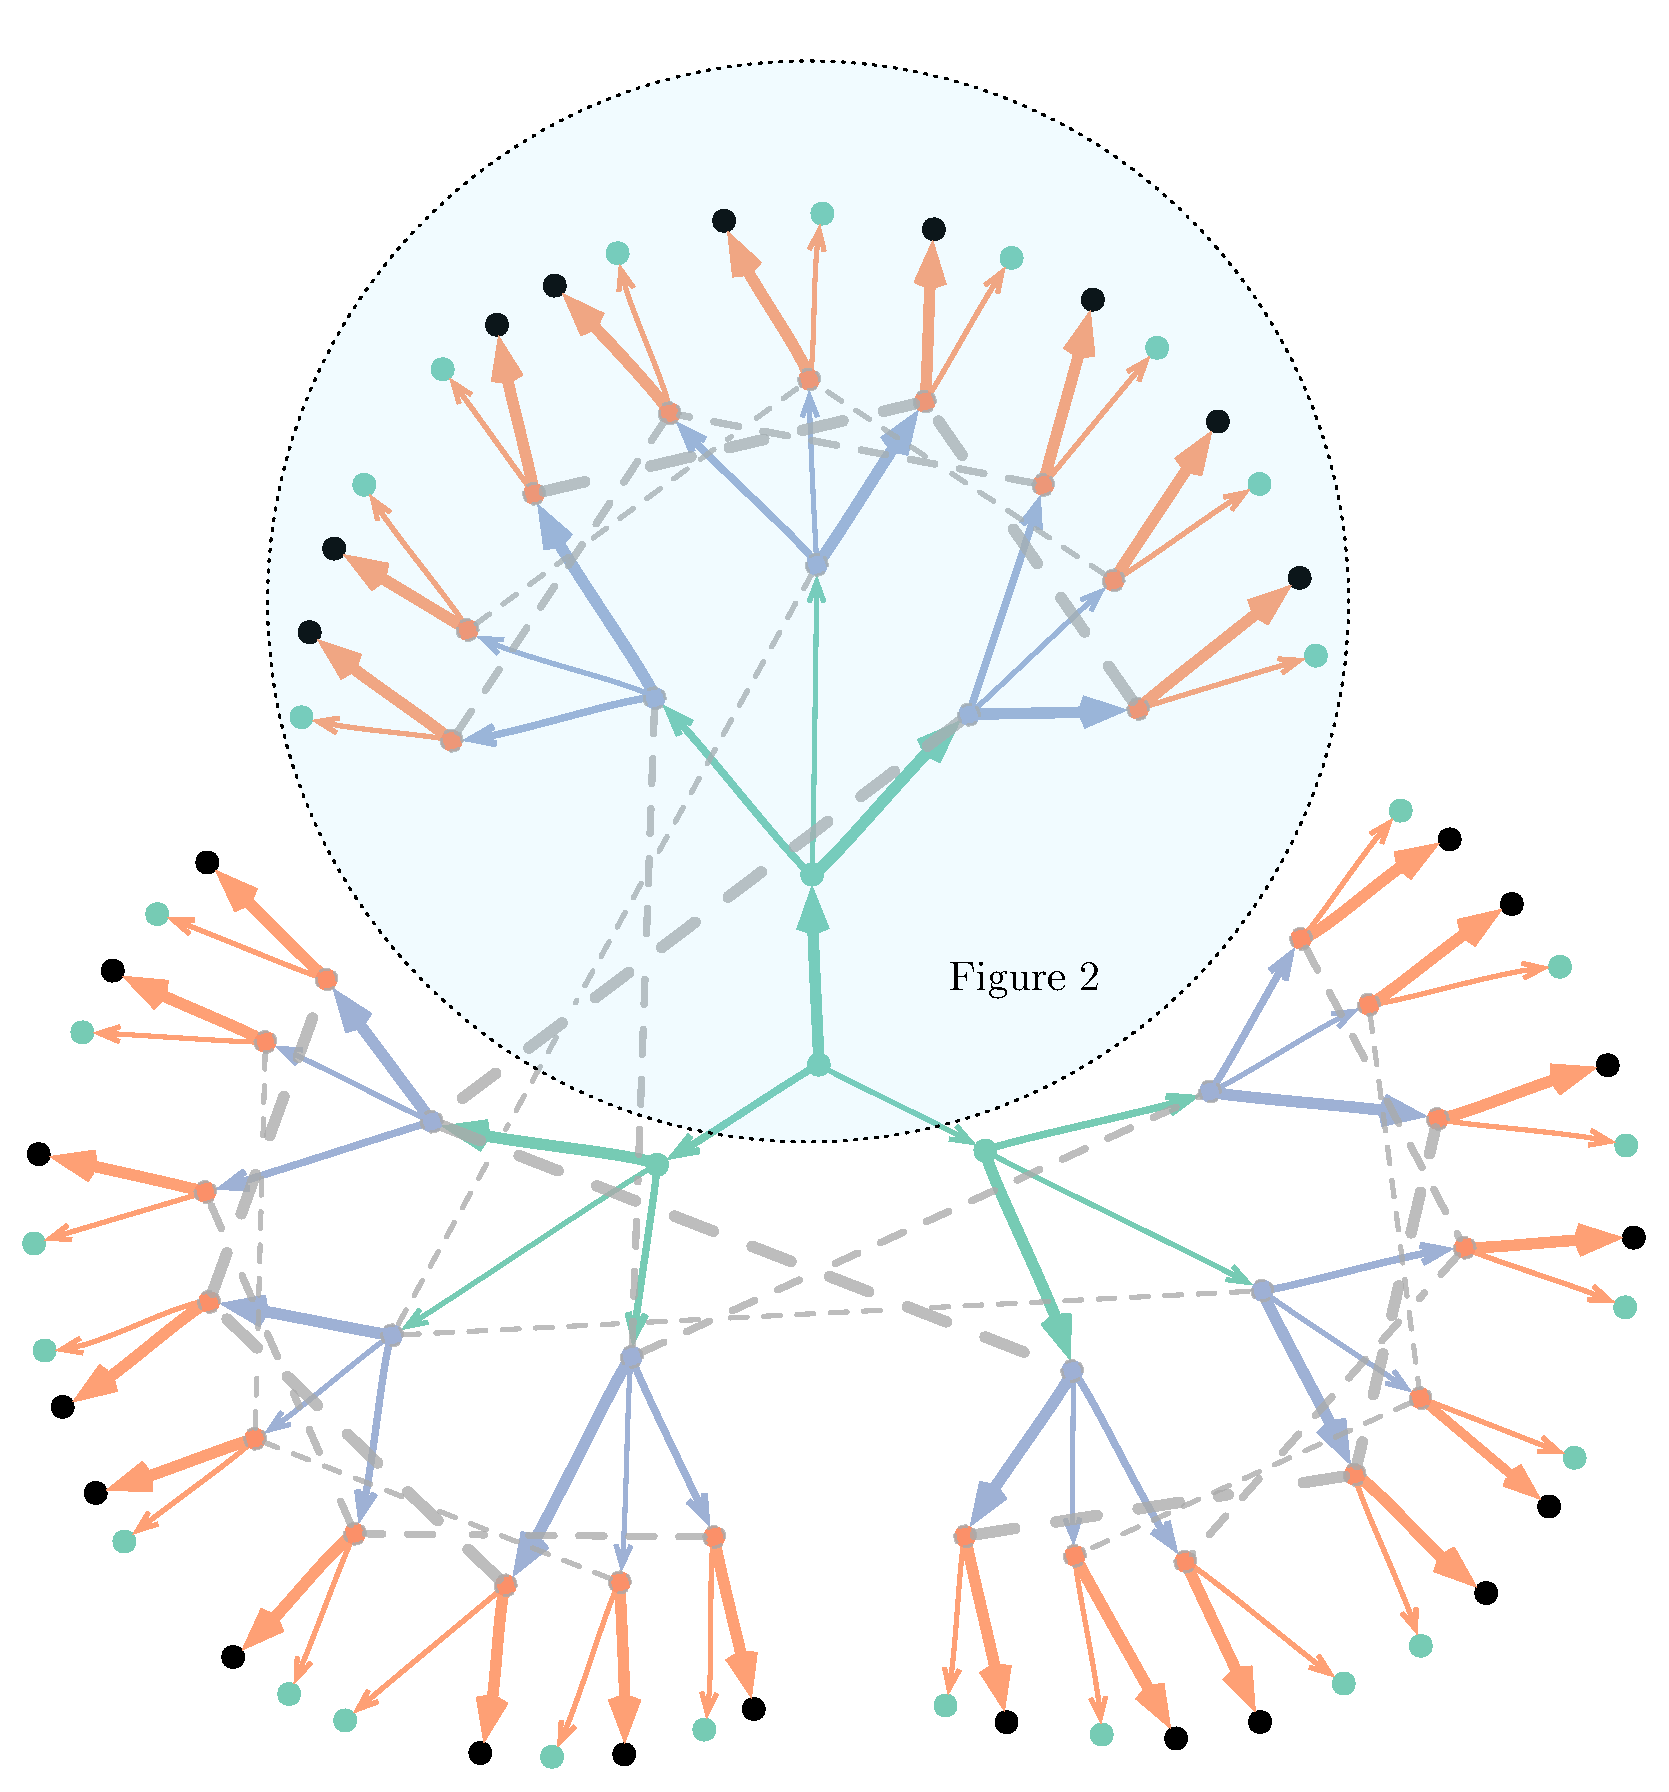
\includegraphics[width=119mm]{figures/rounded_clover_infosets}
\end{adjustbox}
\caption{Simplified game tree. Arrows correspond to two moves by nature, followed by women, and midwives respectively. Line weight distinguishes between information sets, and possible moves, corresponding to ascending player types. For midwives, referral is shown by a heavier arrow. Light terminal nodes indicate that the game may repeat from that point, and black nodes are exits}

\label{fig:simple_tree}
\end{figure}

\begin{figure}[H]
\begin{adjustbox}{center}
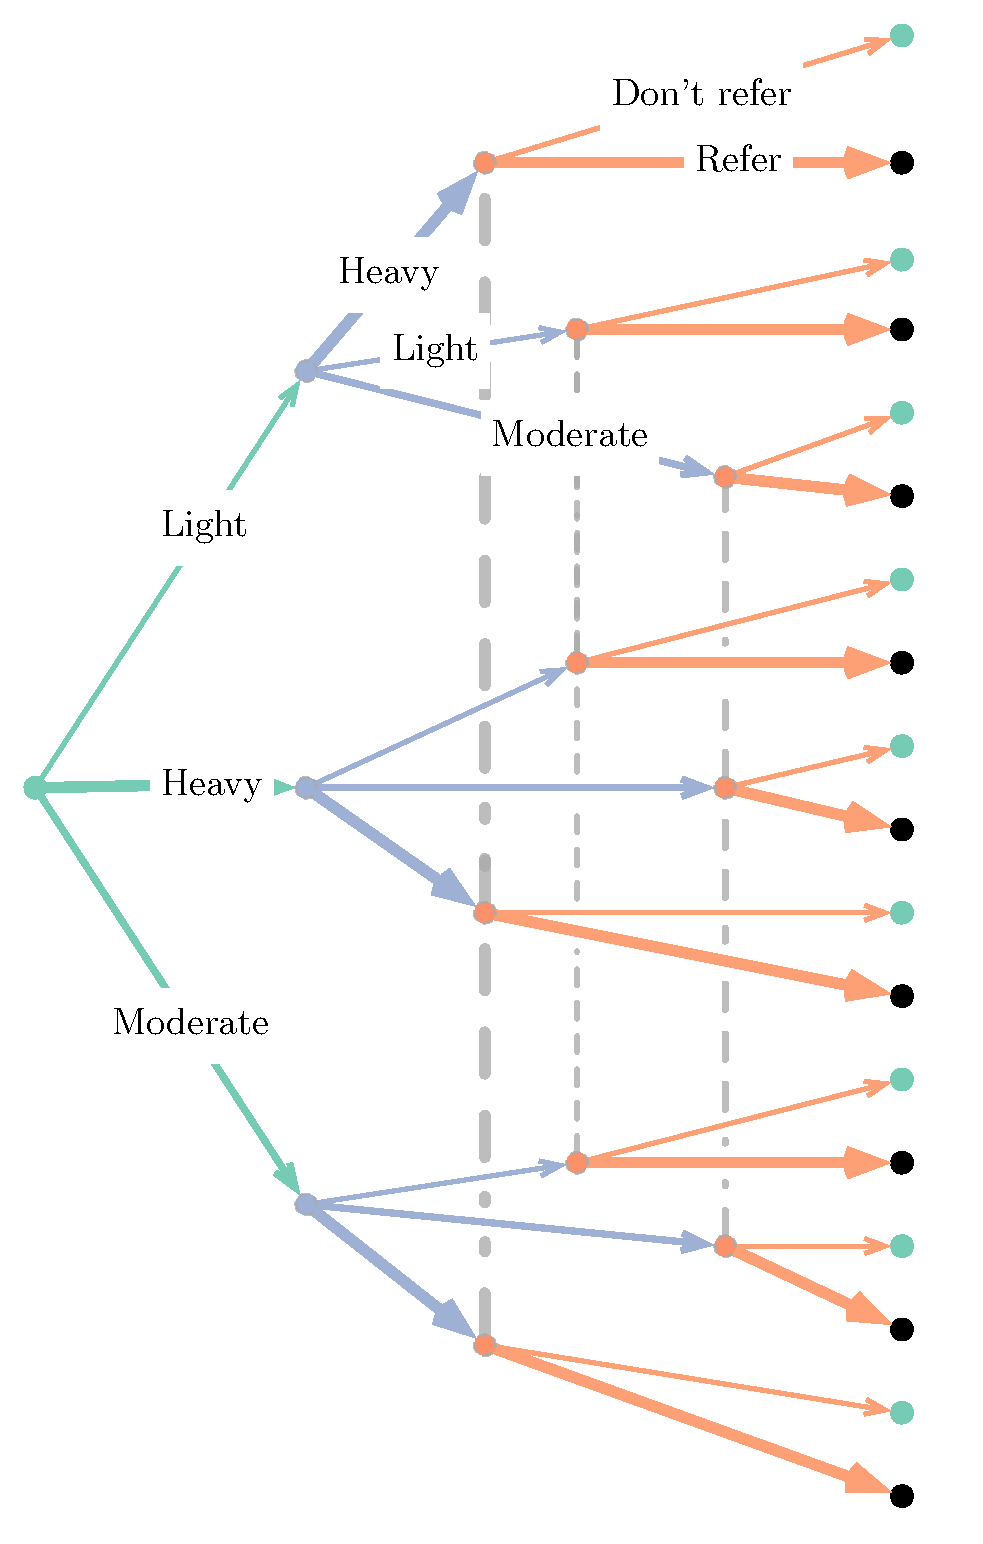
\includegraphics[width=119mm]{figures/tree_zoom}
\end{adjustbox}
\caption{Detail view of a single game tree branch, showing the possible moves by each player, with information sets for midwives}

\label{fig:zoom_tree}
\end{figure}

%Might belong in a more methody bit? Read some stuff to check..
To formally define the game, let \(N = \{m, w\}\) be the set of players each with a private type \(\theta_{i} \in \Theta\), and a set of types \(\Theta=\{l, m, h\}\), with pure strategies \(A_{m}=\{r,n\}, A_{w}=\{l, m, h\}\). Here, \(\{l, m, h\}\) correspond to light, moderate, and heavy alcohol consumption for women, and non-judgemental, moderately judgemental, and harshly judgemental for midwives. Midwives' pure strategies \(\{r,n\}\) are to refer, or do nothing, and those for women are to signal that they have one of the possible drinking patterns.
Additionally define two utility functions - 
\begin{equation}
u_{w}(s_{w}, s_{m}, \theta_{w}, \theta_{m})=X_{s, s_{w}, \theta_{m}} + X_{h, \theta_{w}, s_{m}}
\end{equation} 
\begin{equation}
u_{m}(s_{w}, s_{m}, \theta_{w})=X_{h, \theta_{w}, s_{m}} + X_{c, \theta_{w}, s_{m}},
\end{equation} with $X_{c}$, $X_{h}$, and $X_{s}$ being the payoff matrices as in table \ref{tab:Payoff-matrix}, $s_{w}$ and $s_{m}$ denoting a specific signal by a woman, and referral response by a midwife. Lastly let \(p_{w}(l, m, h)\), \(p_{m}(l, m, h)\) be distributions over types of women, and midwives respectively.


As noted, rather than solve the game, we allow populations of agents to play it, and hence stipulate further that women are drawn in order from a queue of \(n_{w}\) women (where \(n_{w}=1000\) in all simulations), and play against a midwife chosen at random from a population of \(n_{m}\) (\(n_{m}=100\)). They play for a maximum of \(r_{w}\) rounds (\(r_{w}=12\) following the routine number of ante-natal appointments in the UK \citep{NICE2010a}) or until they are referred, and a new player is drawn from the same distribution that produced the original players to replace them. If they are not referred, they rejoin the back of the queue after their appointment. In either case, they are informed of their payoff after each round and update their beliefs accordingly using one of the rules described in section \ref{sub:the_agents}.

Midwives play for \(r_{m}\) rounds (\(r_{m}=1000\) in all experiments), and conduct appointments in parallel, i.e. if there are 5 midwives, then five women are drawn from the queue and assigned at random to the midwives. 
Unlike women, midwives are only informed of their payoff if they choose to make a referral. Both groups of agents have perfect recall, and midwives are assumed to retrospectively update their observations if they make a referral after a number of appointments.
\end{comment}